Ниже продемонстрированы результаты работы программного кода написанного на Python.


Волновая функция основного состояния, полученного методом Ритца и её плотность представлены на Рис.~\ref{fig:State0PB}

\graphicspath{{../python_results}}

\begin{figure}[h]
\centering
    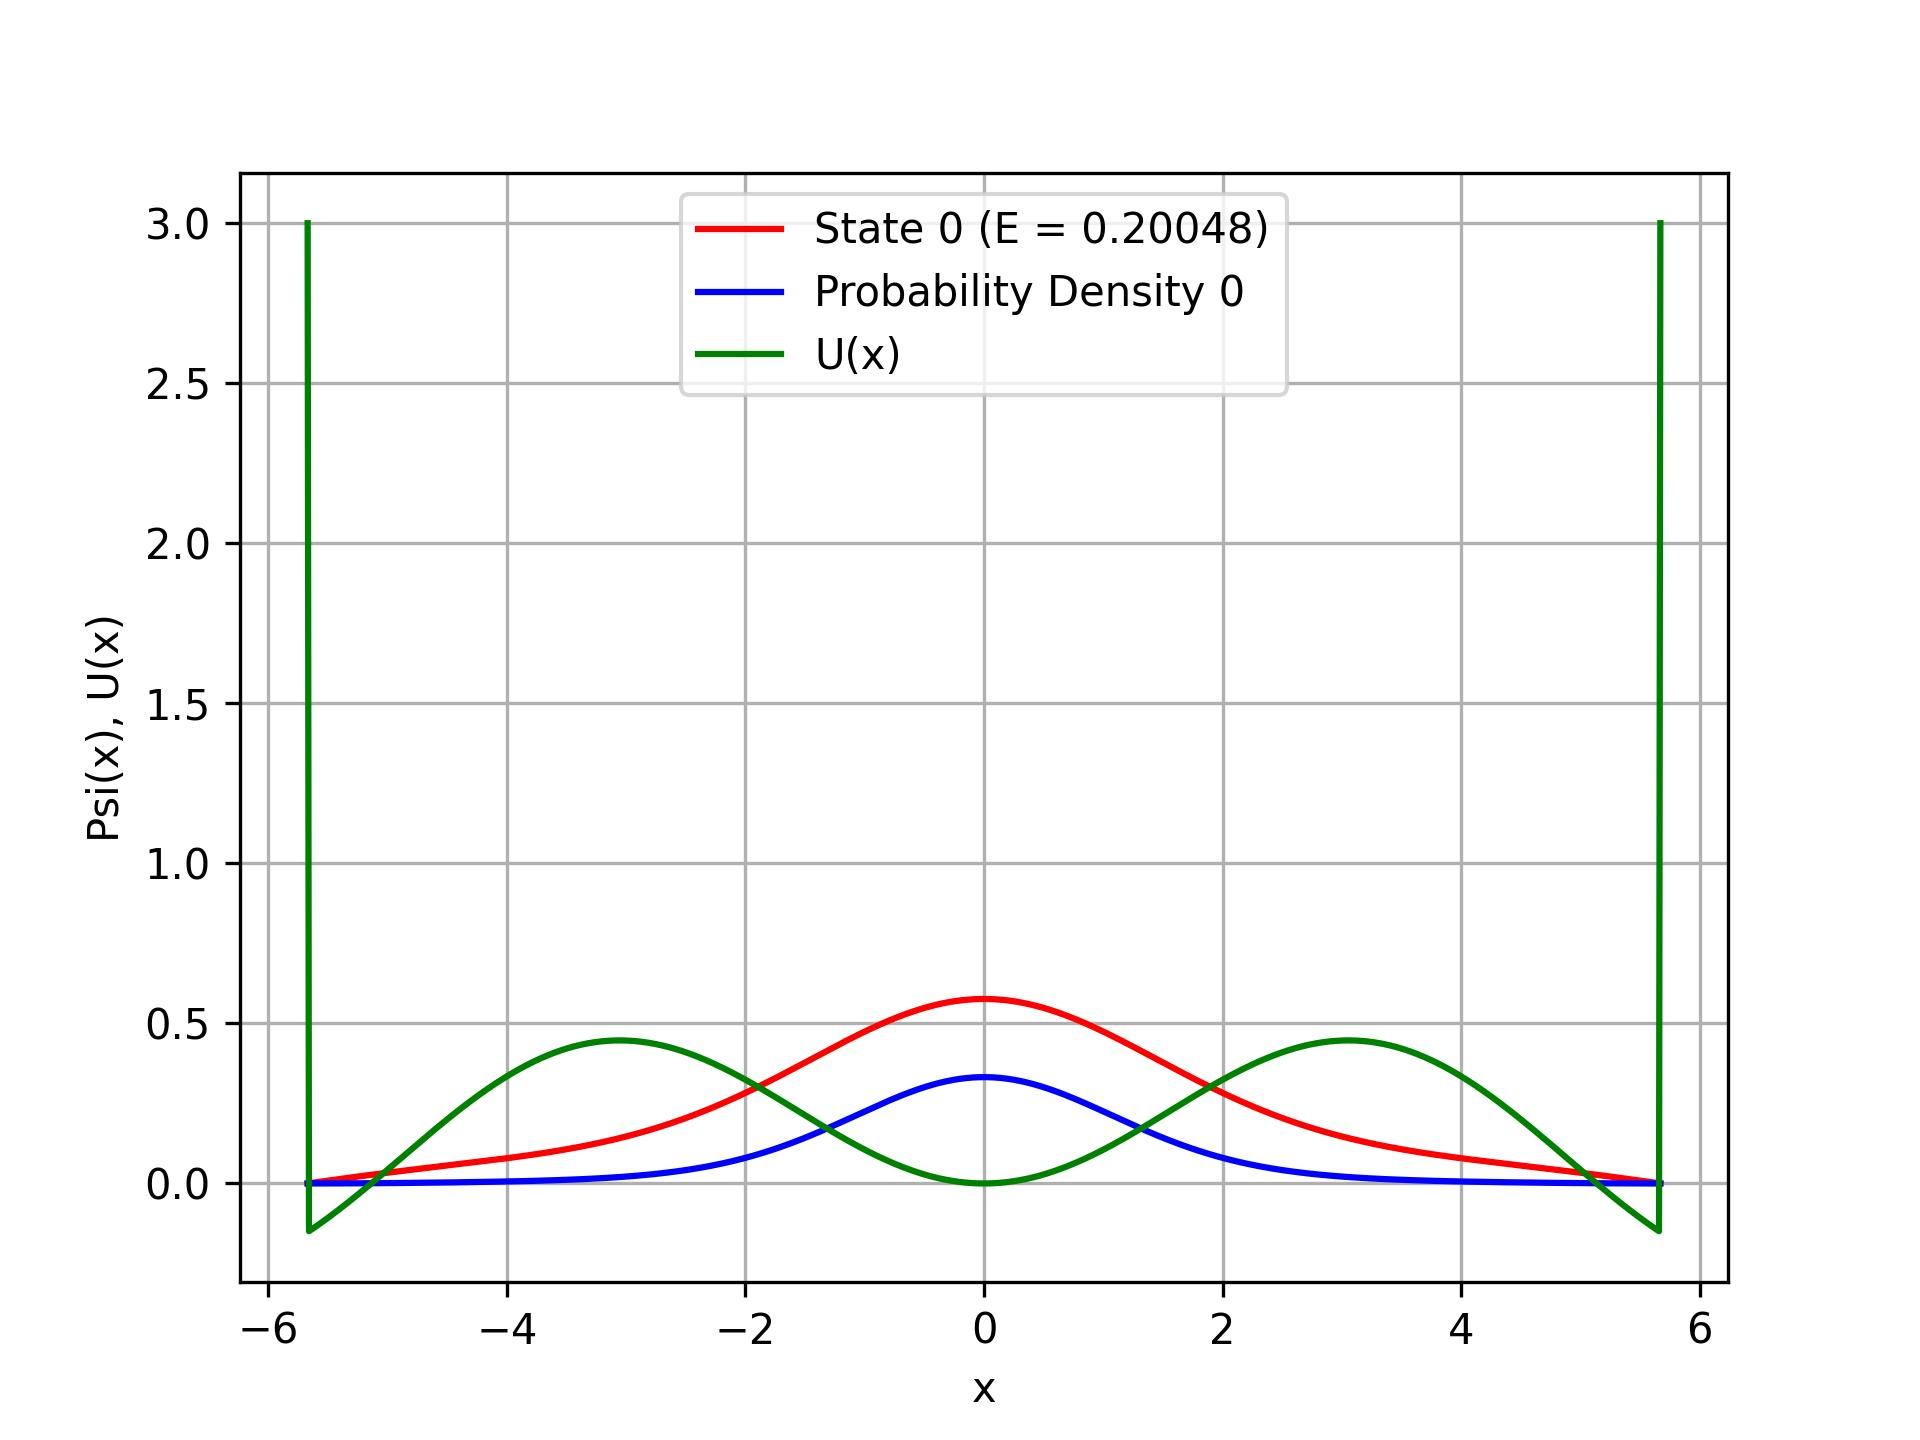
\includegraphics[width=0.6\linewidth]{State 0 probability density}
    \caption{Волновая функция основного состояния, полученная методом Ритца}\label{fig:State0PB}
\end{figure}

Волновая функция, полученная данным методом, согласно осцилляционной теореме соответствует основному состоянию.

Сравним волновые функции основного состояния, полученные методом Ритца и методом пристрелки (Рис.~\ref{fig:State0}):

\begin{figure}[h]
\centering
    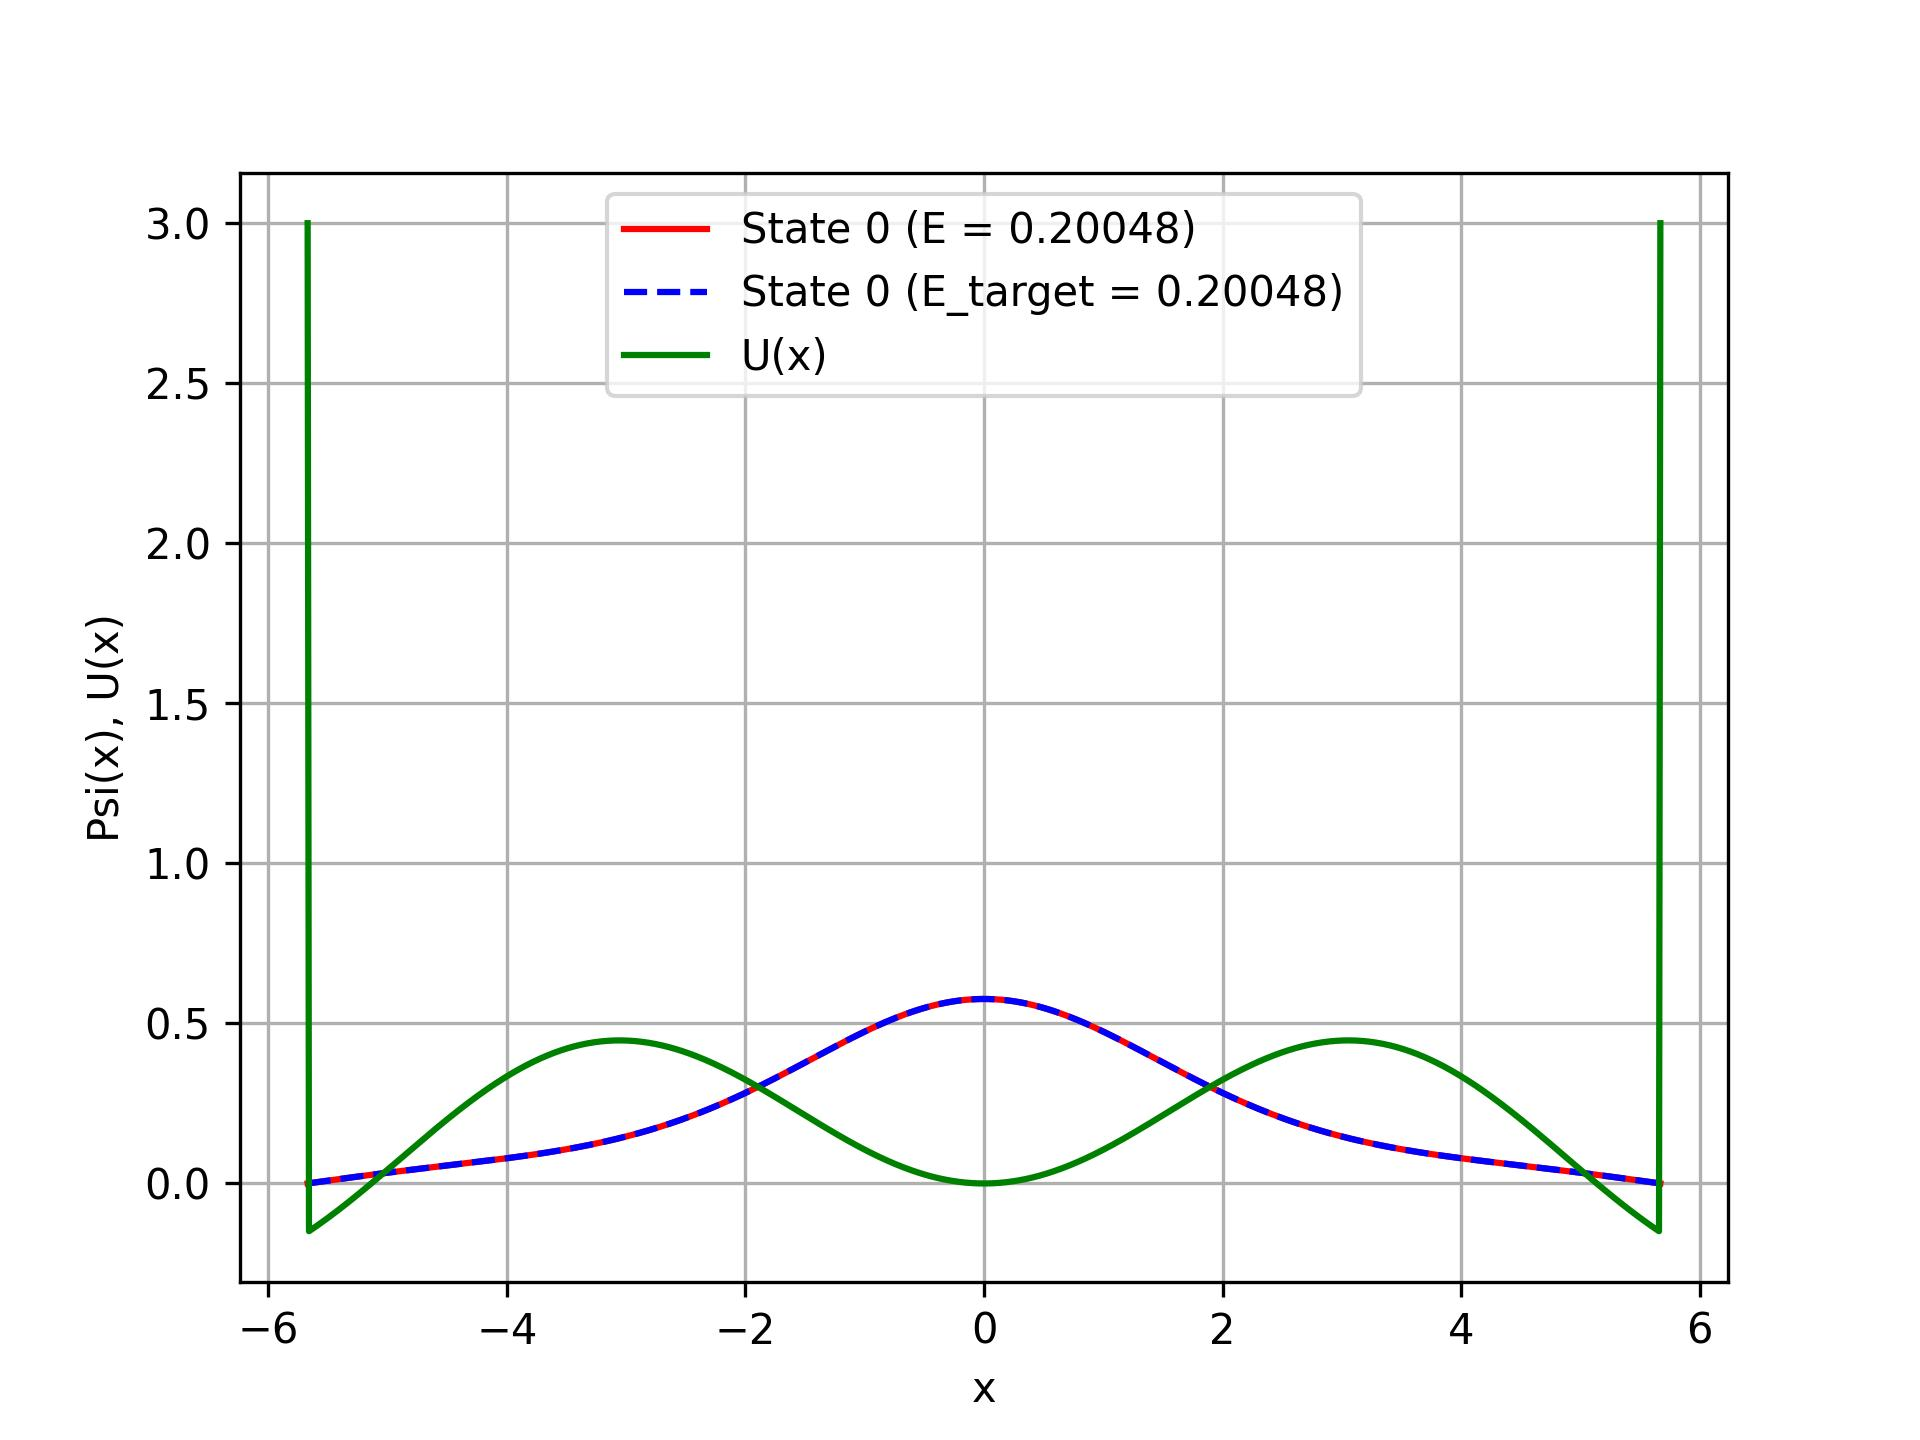
\includegraphics[width=0.6\linewidth]{State 0}
    \caption{Волновая функция основного состояния, сравнение методов}\label{fig:State0}
\end{figure}


Как можно заметить, данные функции не сходятся, даже более того - функция, полученная методом Ритца, имеет 0 пересечений с осью абсцисс,
в то время как функция, полученная методом пристрелки имеет два пересечения.
Как было рассмотрено в предыдущих лабораторных работах -- основным состоянием для заданной потенциальной функции является состояние с индексом $k=2$.
Предположим, что данный метод либо не подходит для решения текущей задачи (задача в которой основное состояние начинается с $k=2$).

Рассмотрим следующие состояния, полученные текущими методами.

\begin{figure}[H]
    \centering
    \begin{subfigure}{0.45\textwidth}
        \centering
        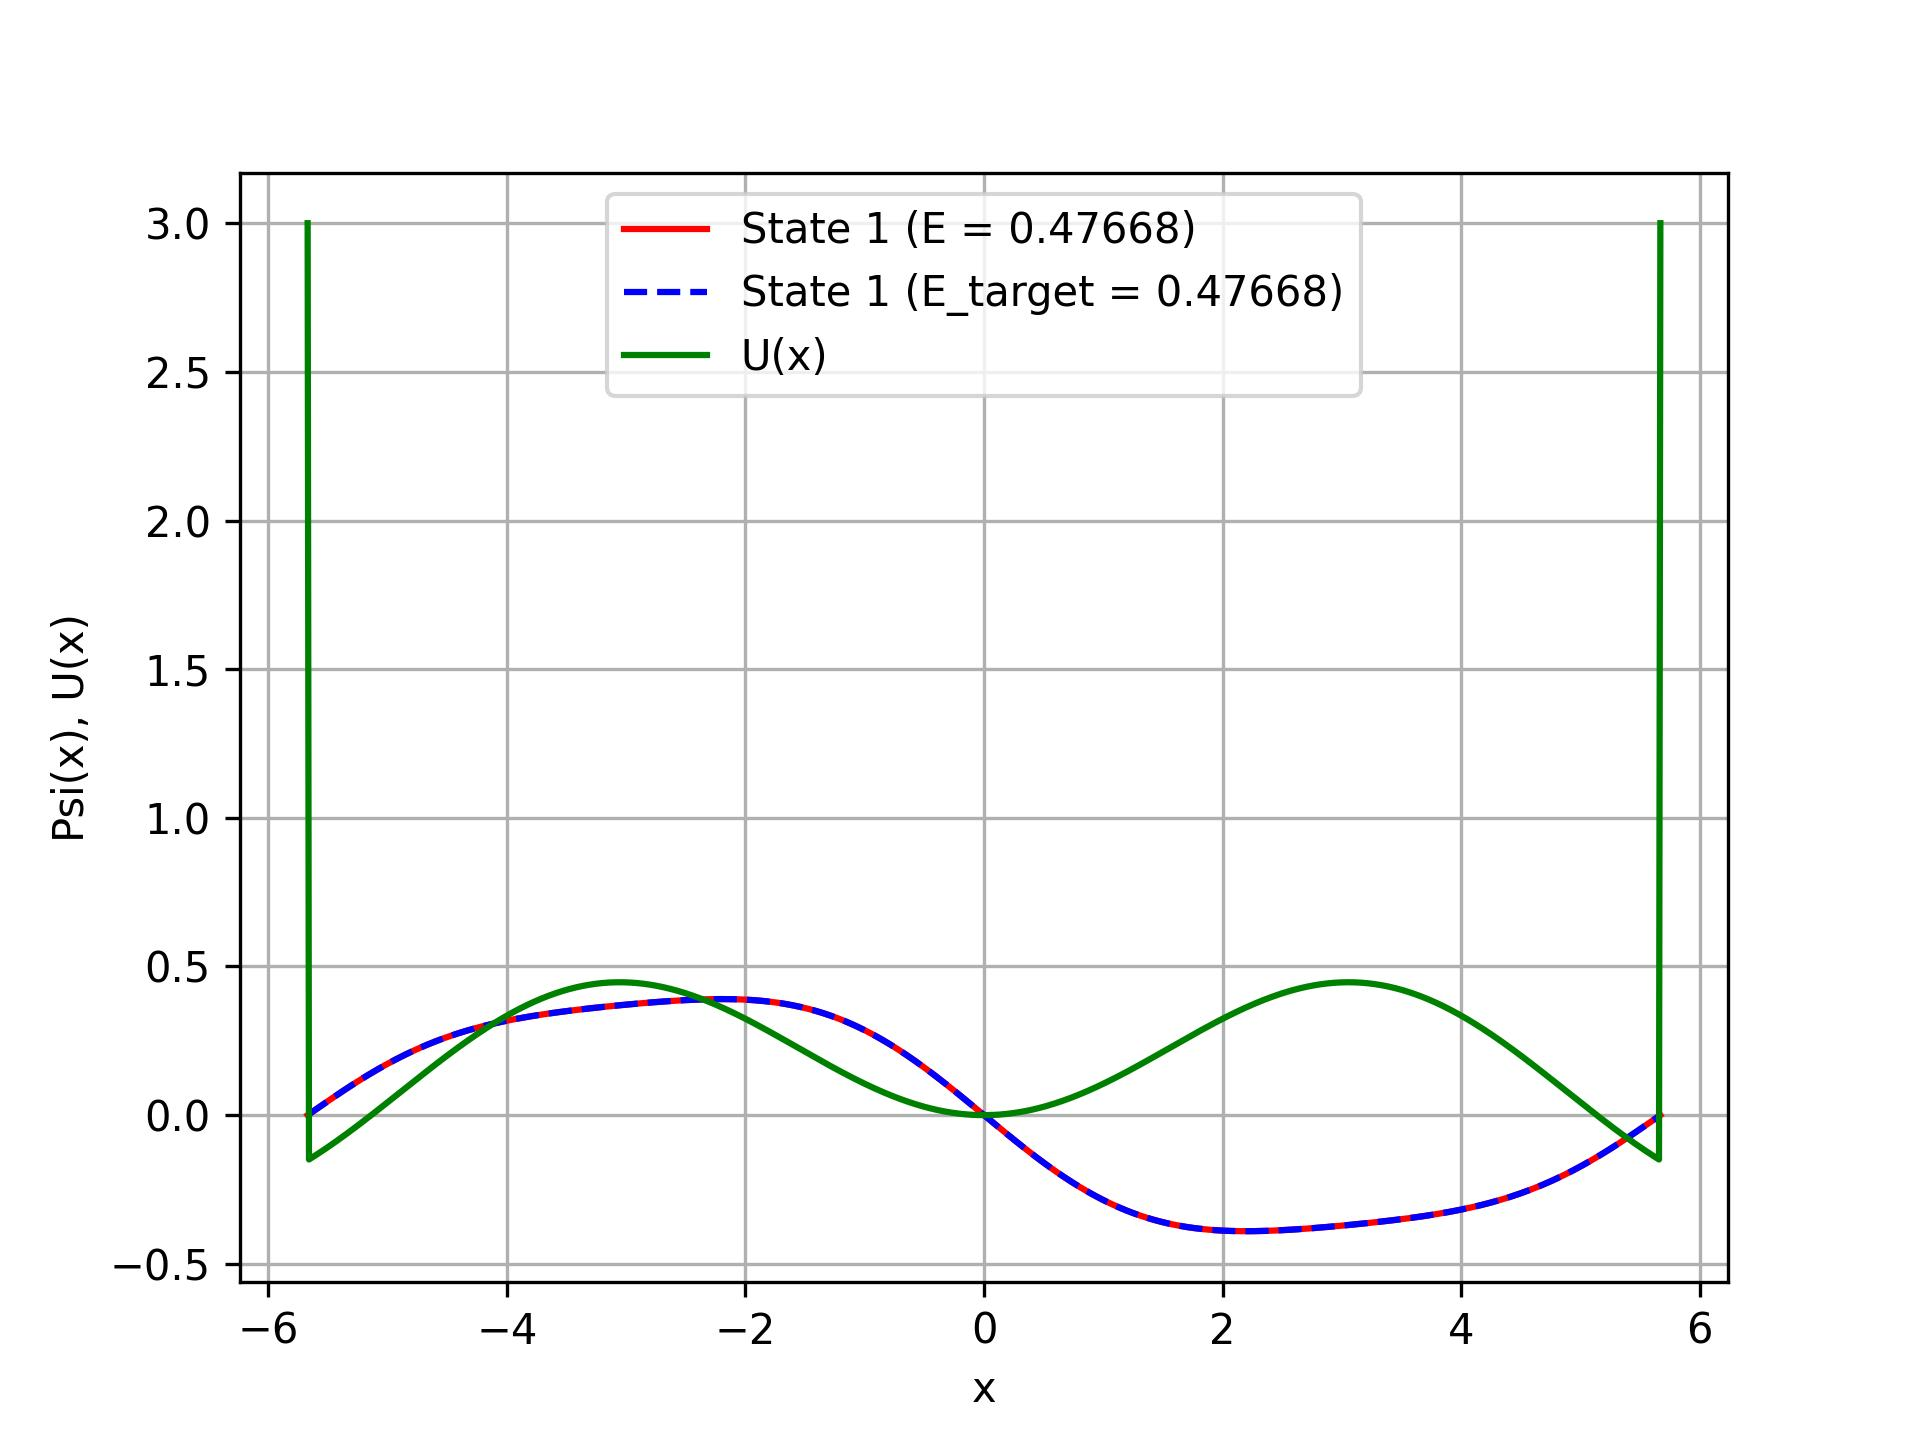
\includegraphics[width=0.9\linewidth]{State 1}
        \caption{Состояние 1}
        \label{fig:state1}
    \end{subfigure}%
    \begin{subfigure}{0.45\textwidth}
        \centering
        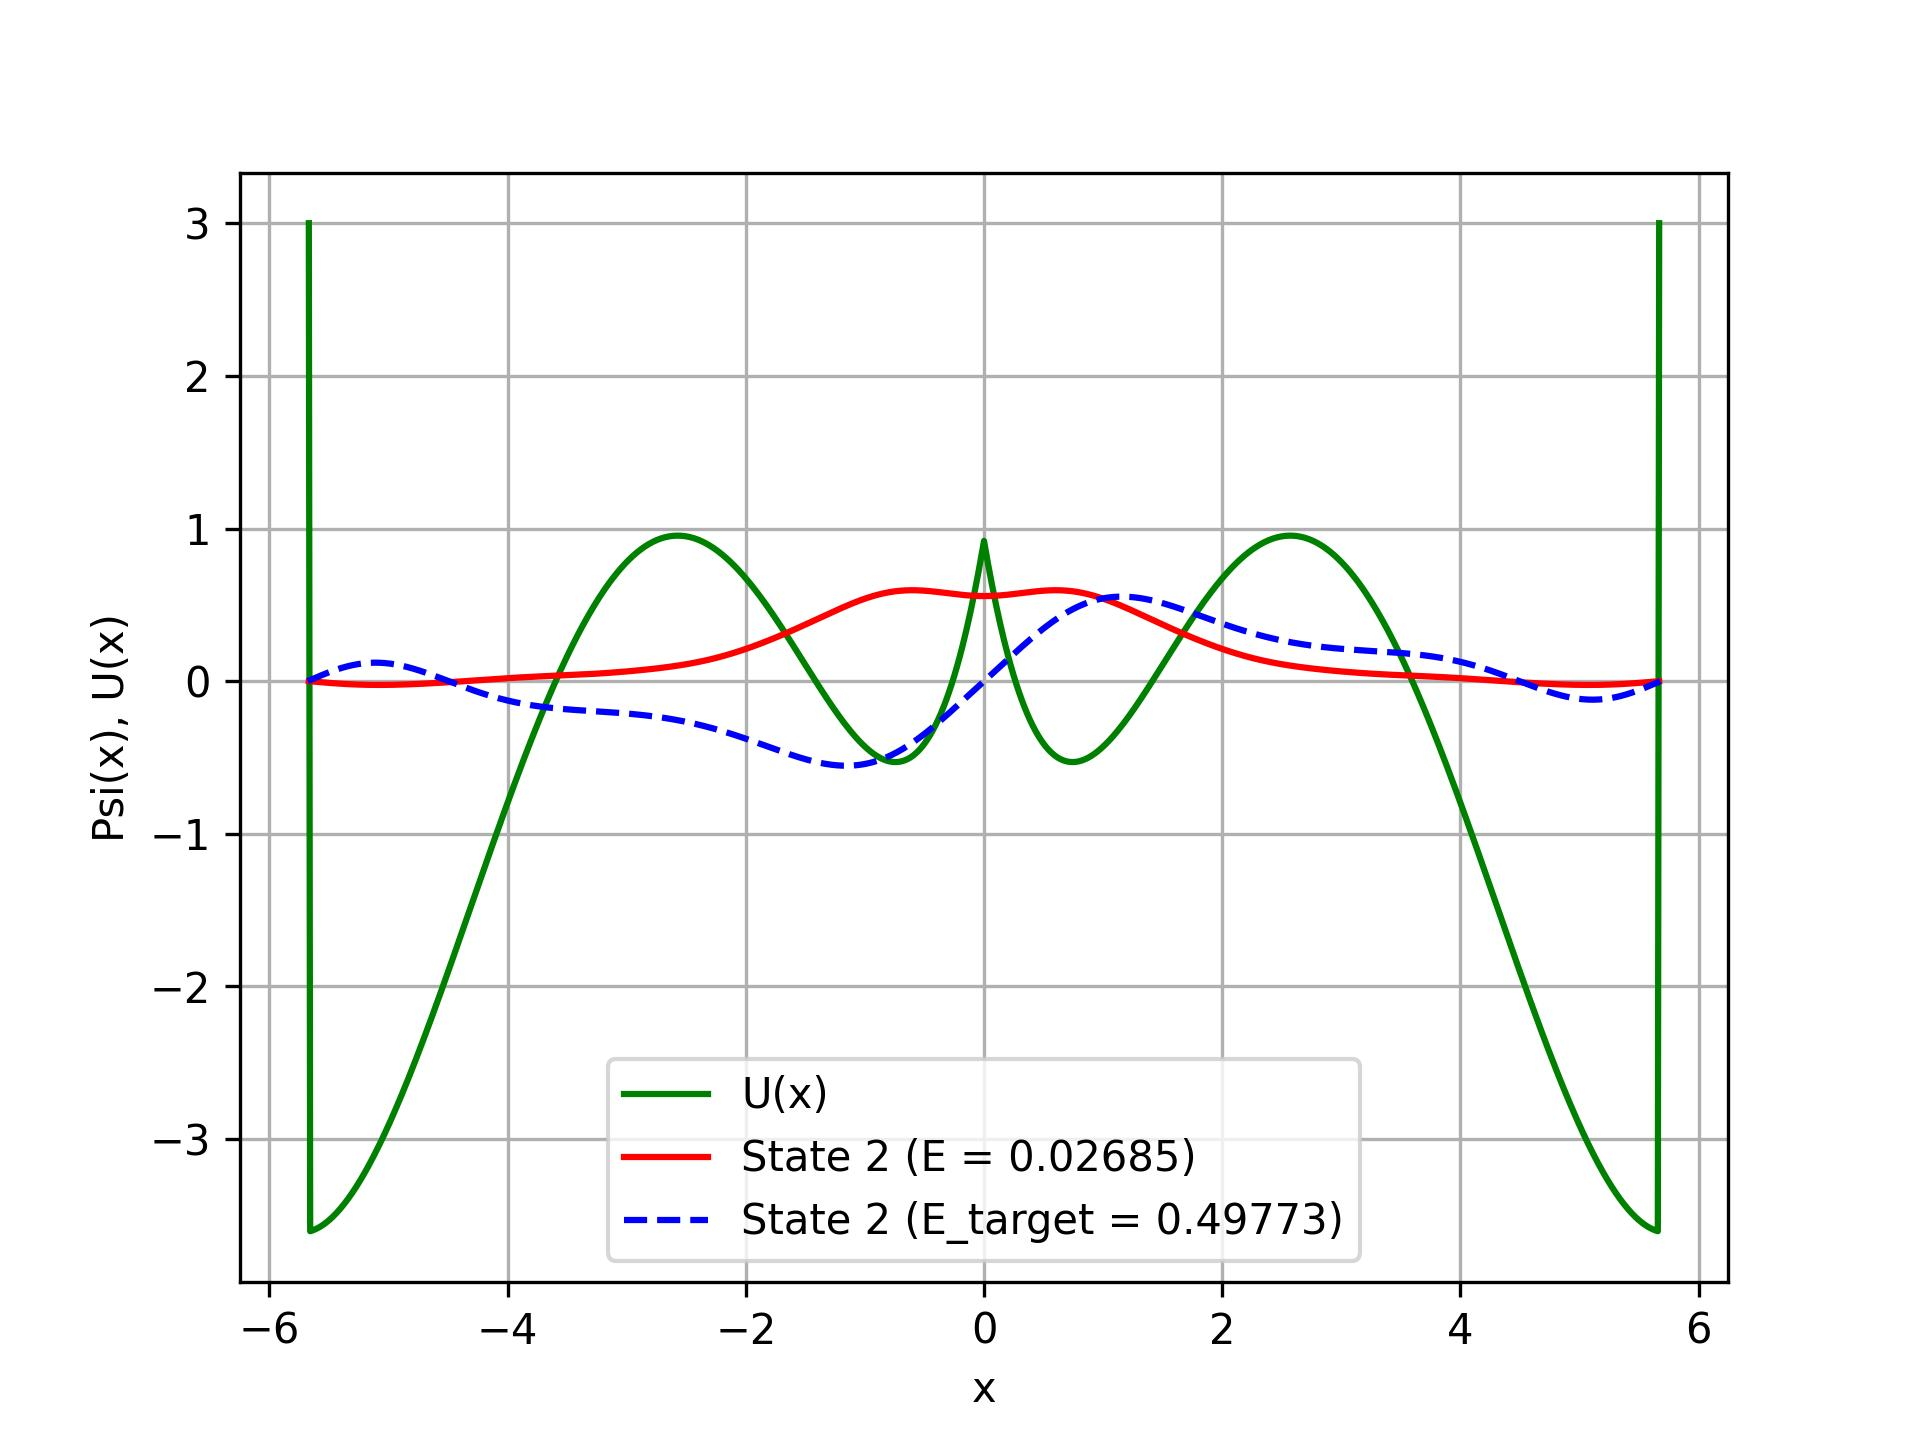
\includegraphics[width=0.9\linewidth]{State 2}
        \caption{Состояние 2}
        \label{fig:state2}
    \end{subfigure}%
\caption{Графики для состояний 1 и 2}
\end{figure}
\label{fig:state12}
Как можно заметить, в обоих случаях графики функций разнятся.
Сравним энергии, полученные в процессе решения задачи методом Ритца и методом пристрелки:
\begin{table}[H]
    \centering
    \noindent
    \begin{tabularx}{\linewidth}{|X|X|X|}
        \hline
        \textbf{Состояние}&\textbf{Метод Ритца энергия, а.е.}&\textbf{Метод пристрелки энергия, а.е.}\\
        \hline
        Основное & $-1.264468$ & $0.026429199218641876$\\
        \hline
        1-е возбужденное & $-1.264465$ & $0.49773486328114225$\\
        \hline
        2-е возбужденное & $0.026845$ & $0.8155639648436425$\\
        \hline
        3-е возбужденное & $0.498926$ & $0.9052211914061424$\\
        \hline
        4-е возбужденное & $0.828370$ & $2.0405639648435283$\\
        \hline
    \end{tabularx}\label{tab:energies}
\end{table}

Как можно заметить, энергии, полученные методом Ритца и методом пристрелки разнятся, однако,
также можно заметить что данные энергии сходятся, но для разных состояний.
Имеет смысл предположить что в силу большей точности метод Ритца позволяет найти значения энергий,
которые метод Пристрелки даст только с крайне малым шагом $\triangleE$,
при котором вычисления будут производиться значительно большое количество времени.

%Подытожив, выведем энергии полученные для первых двух состояний (включая основное) разными методами,
%а также квантовомеханические средние $\langle p(x) \rangle$ и $\langle p(x^2) \rangle$
%
%
%\noindent
%\begin{tabularx}{\linewidth}{|c|c|X|X|X|}
%    \hline
%    \textbf{Метод}&\textbf{Состояние}&\textbf{Энергия, а.е.}&\textbf{$\langle p(x) \rangle$}&\textbf{$\langle p(x^2) \rangle$} \\
%    \hline
%    Ритца & Основное & $-1.264468$ & $0.000000e+00$ & $3.070530e-01$ \\
%    \hline
%    Пристрелки & Основное & $-1.283224$ & $0.000000e+00$ & $3.070530e-01$ \\
%    \hline
%    Ритца & 1-е возбужденное & $0.815564$ & $0.000000e+00$ & $2.435363$ \\
%    \hline
%    Пристрелки & 1-е возбужденное & $0.815564$ & $0.000000e+00$ & $2.435363$ \\
%    \hline
%    Ритца & 2-е возбужденное & $0.815564$ & $0.000000e+00$ & $2.435363e+00$\\
%    \hline
%    Пристрелки & 2-е возбужденное & $0.815564$ & $0.000000e+00$ & $2.435363e+00$\\
%    \hline
%\end{tabularx}
\newpage